\section{Modello}
L'unità di calcolo fondamentale in NNAPI è il modello, il quale è definito da uno o più operandi e operazioni.
Gli operandi sono data object utilizzati nella definizione del grafo, tra i quali costanti, input, output e nodi intermedi; possono essere di due tipi: scalari e tensori.
Uno scalare è un singolo valore in uno dei vari formati booleano, intero o virgola mobile a 16/32 bit.
I tensori, invece, sono array n-dimensionali. In NNAPI i tensori possono anche essere quantizzati a 8 o 16 bit.

\begin{figure}[ht]
    \centering
    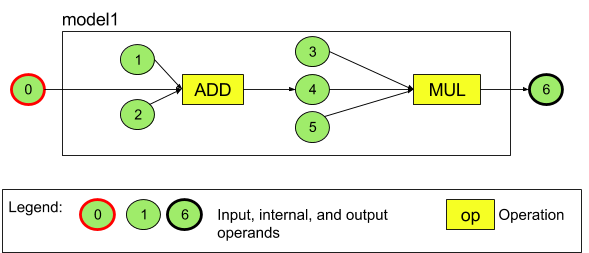
\includegraphics[width=0.7\textwidth]{Immagini/operandi.png}
    \caption{Esempio di operandi per un modello NNAPI}
    \label{fig:operandi}    
\end{figure}

\subsection{Fasi operative}
In NNAPI, un'operazione specifica i calcoli da eseguire ed è costituita dai seguenti elementi:
\begin{itemize}
    \item il tipo di operazione (ad es. addizione, moltiplicazione, convoluzione);
    \item l'elenco di indici degli operandi utilizzati dall'operazione per l'input;
    \item l'elenco di indici degli operandi utilizzati dall'operazione per l'output.
\end{itemize}
Prima di aggiungere l'operazione, bisogna aggiungere al modello gli operandi utilizzati o prodotti da questa operazione.

L’utilizzo delle Neural Networks API avviene a basso livello, grazie a linguaggi come C/C++. In particolare C++ rispecchia la programmazione ad oggetti (come lo sono Java e Kotlin) e permette quindi di
definire veri e propri modelli come oggi in maniera intuitiva.
Per creare un modello, per esempio, basta definire due righe di codice:
\begin{center}
\texttt{ANeuralNetworksModel\* model = NULL;} \\ \texttt{ANeuralNetworksModel\_create(\&model);}\\
\end{center}
Dopo la creazione è necessario aggiungere i vari operandi attraverso \texttt{ANeuralNetworks\_addOperand()} e sfruttando le strutture dati fornite, come \textit{ANeuralNetworksOperandType}.

\section{Compilation}
In questa fase viene determinato su quali processori verrà eseguito il modello e viene chiesto ai driver corrispondenti di preparasi per l’esecuzione di questo, eventualmente generando anche codice macchina specifico per i processori scelti.
Da sottolineare la possibilità di scegliere esplicitamente quali dispositivi utilizzare e il tradeoff tra l’utilizzo della batteria e la velocità di esecuzione.

\subsection{Esecuzione Sincrona VS Asincrona}
Alcune operazioni nel runtime NNAPI sono eseguite in maniera sincrona. Ciò significa che ogni operazione di questo tipo può rallentare l’esecuzione di un'altra operazione in attesa del risultato,
in quanto è necessario attendere la fine dell'esecuzione per continuare l'esecuzione; in questo modo viene ridotta la potenza innata del multithreading.

Di contro, sfruttare esecuzioni asincrone non sempre è conveniente, in quanto il dispositivo deve poter generare e sincronizzare tutti i vari thread, con latenza variabile. A volte è possibile avere ritardi di più di
500 microsecondi tra quando viene inviata la notifica di un thread al momento in cui viene associato un core. 

Da Android 10 in poi, NNAPI supporta le \textit{burst executions} tramite l'uso di un oggetto apposito. Queste esecuzioni altro non sono che sequenze di esecuzioni della stessa compilazione che si verificano in rapida successione,
come la campionatura audio o l’acquisizione video. Gli oggetti burst quindi possono portare ad esecuzioni più rapide, dove gli acceleratori rimangono in uno stato di prestazioni elevate per tutta la durata del burst.

\subsection{Gestione errori}
Di norma, se si verifica un errore durante il partizionamento o un errore con i driver scelti, NNAPI ricorre alla implementazione della CPU per una o più operazioni ove possibile. Sfruttando framework come TensorFlow Lite,
nella maggior parte dei casi, può essere vantaggioso disabilitare il ricorso all'utilizzo della CPU e gestire gli errori con implementazioni delle operazioni ottimizzate dal client.

Se il partizionamento o la compilazione non vanno a buon fine, l’intero modello sarà provato sulla CPU, stessa cosa vale per un’operazione che continua a fallire. Questo ovviamente riduce notevolmente la velocità
di esecuzione ma aumenta le possibilità di successo, riducendo eventuali errori hardware. Da considerare, però, che alcune operazioni non sono nemmeno supportate dalla CPU.
È possibile quindi disabilitare il fallback della CPU e rimuoverla dall’elenco dei processori nel caso in cui non la si voglia utilizzare per le operazioni del modello.

\subsection{Memoria}
Da sottolineare la possibilità, da Android 11 e successive, di sfruttare domini di memoria che forniscono interfacce di allocazione per memorie opache (sono un tipo di memoria che è gestita in modo che i dettagli interni non siano
direttamente accessibili o modificabili dall'utente o dalle applicazioni). Ciò permette alle applicazioni di passare dati e ricordi nativi del dispositivo tra le varie esecuzioni, in modo che NNAPI non copi o trasformi i dati
inutilmente quando vengono effettuate esecuzioni consecutive sullo stesso driver.
Queste funzionalità sono destinate principalmente ai tensori interni ai driver con pochi accessi lato client, come i tensori di stato. Per tensori con frequenti accessi alla CPU lato client, è necessario utilizzare pool di memoria condivisi.

\section{Tempo di esecuzione}
Il test delle prestazioni di un'app può essere effettuato misurando il tempo di esecuzione o tramite profilazione. Per misurare il tempo di esecuzione, si può utilizzare l'API di esecuzione sincrona o API a livello inferiore
come \textit{ANeuralNetworksExecution\_setMeasureTiming} e \textit{ANeuralNetworksExecution\_getDuration}. Queste API consentono di misurare il tempo di esecuzione su un acceleratore o nel driver, escludendo l'overhead dovuto al runtime NNAPI
e all'IPC.

Le informazioni di tempistica possono essere utili per ottimizzare le prestazioni dell'applicazione in produzione, anche se la raccolta di tali informazioni potrebbe influenzare le prestazioni stesse (cosa da notare in fase di
controllo e revisione dei dati). È importante notare che solo il driver è in grado di calcolare il tempo trascorso su se stesso o sull'acceleratore.

Per profilare l'applicazione, si può utilizzare \textit{Android Systrace}, che genera automaticamente eventi \texttt{systrace} per profilare diverse fasi del ciclo di vita del modello e i vari livelli dell'applicazione, come Application,
Runtime, IPC e Driver.
Per generare i dati di profilazione NNAPI, è possibile utilizzare il comando systrace di Android e l'utility \texttt{parse\_systrace}. Questi strumenti consentono di analizzare gli eventi systrace generati dall'applicazione e di ottenere
una visualizzazione tabellare dei tempi spesi nelle diverse fasi del ciclo di vita del modello e nei diversi livelli dell'applicazione.
Inoltre, Android 11 introduce miglioramenti nella qualità del servizio (QoS) per NNAPI, consentendo alle applicazioni di indicare le priorità relative dei propri modelli e di impostare timeout per la compilazione e l'inferenza del modello.

Infine, sono disponibili argomenti avanzati sull'utilizzo degli operandi NNAPI, come tensori quantizzati, operatori facoltativi e tensori di ranking sconosciuto. Il benchmark NNAPI è disponibile su AOSP per valutare latenza e accuratezza
dei modelli.

\subsection{Log}
NNAPI offre informazioni diagnostiche utili nei log di sistema, che possono essere analizzati utilizzando l'utilità logcat. È possibile attivare il logging dettagliato per fasi o componenti specifici impostando la proprietà
\textit{debug.nn.vlog} tramite adb shell. Questo consente di registrare informazioni dettagliate su fasi come la creazione di modelli, la compilazione, l'esecuzione e altro ancora.
Una volta attivato, il logging dettagliato genererà voci di log con un tag impostato sul nome della fase o del componente. Per controllare il livello dei messaggi di log mostrati da logcat si utilizza
la variabile di ambiente \textit{ANDROID\_LOG\_TAGS} (è solo un filtro applicato a logcat, si deve comunque impostare la proprietà debug.nn.vlog su all per generare informazioni di log dettagliate).

